\chapter{Applications of Fourier duality}
\label{chap-applications-trans-fourier-grpe-finite}
\chapteroverview{Character theory connects problems that initially look quite
different: quadratic residues, fast transforms on binary data, and the weight
distribution of a code. We develop Gauss sums and quadratic reciprocity,
construct the Walsh transform, and derive Poisson summation and the MacWilliams
identity. The exercises connect these ideas to wavelets, compression, and
sampling.}

\section{Gauss sums}
\label{sect1-are-gauss}
A finite field has both an additive group and a multiplicative group.
Gauss sums combine their characters and reveal how the two structures
interact. For a detailed treatment of finite fields and character sums, see
Lidl and Niederreiter~\cite{lidl} and Langevin~\cite{langevin}.

\subsection{Quadratic residues}
Consider the integer equation
\begin{equation}
\label{eq-example-quadratic-equation}
 x^2=2y^2+7k,\qquad x,y,k\in\ZZ.
\end{equation}
Modulo $7$, the square roots of $2$ are $3$ and $4=-3$.
If $y\not\equiv0\pmod7$, division by $y^2$ therefore gives
$x\equiv3y$ or $x\equiv4y\pmod7$. If $y\equiv0$, the equation forces
$x\equiv0$ as well. The same conclusion follows uniformly from
\[
 x^2-2y^2\equiv(x-3y)(x-4y)\pmod7.
\]
Thus the integer pairs are exactly those satisfying one of these two
congruences, and $k=(x^2-2y^2)/7$. This does not assert that the rational
number $x/y$ equals an integer of the form $3+7m$ or $4+7m$.

For an odd prime $p$, the \emph{Legendre symbol} records whether an integer
is a square modulo $p$:
\label{notation-25}\index{Legendre symbol}
\[
 \legsymb ap=
 \begin{cases}
 0&p\mid a,\\
 1&a\text{ is a nonzero square modulo }p,\\
 -1&a\text{ is a nonsquare modulo }p.
 \end{cases}
\]
It depends only on the residue class in $\FF_p=\ZZ/p\ZZ$.
Restricted to $\FF_p^*$, it defines the quadratic character
\begin{equation}
\label{eq-defn-cartactere-eta}
 \eta:\FF_p^*\longrightarrow\{1,-1\},\qquad
 \eta(a)=\legsymb ap.
\end{equation}
Its multiplicativity follows from Euler's criterion.

\begin{lem}[Euler's criterion]
\label{lem-formula-euler}
For an odd prime $p$ and $a\in\FF_p^*$,
\[
 a^{(p-1)/2}=\begin{cases}1&a\text{ is a square},\\-1&a\text{ is a nonsquare}.
 \end{cases}
\]
Equivalently, for an integer $a$ not divisible by $p$,
$\legsymb ap\equiv a^{(p-1)/2}\pmod p$.
\end{lem}
\begin{proof}
The homomorphism $x\mapsto x^2$ on $\FF_p^*$ has kernel $\{1,-1\}$,
so its image has $(p-1)/2$ elements. Each square $a=b^2$ satisfies
$a^{(p-1)/2}=b^{p-1}=1$. Since $X^{(p-1)/2}-1$ has at most $(p-1)/2$
roots, these are all its roots. Finally,
$(a^{(p-1)/2})^2=a^{p-1}=1$, so every nonsquare gives $-1$.
\end{proof}
Quadratic reciprocity will relate $\legsymb pr$ and $\legsymb rp$ for distinct
odd primes. Combined with reduction modulo the denominator and the values
of the symbols at $-1$ and $2$, it gives an efficient way to compute
Legendre symbols.

\subsection{Additive and multiplicative characters}
Let $q=p^r$, where $p$ is prime. The field $\FF_q$ has characteristic $p$
and dimension $r$ over its prime subfield $\FF_p$. Its additive group is
isomorphic to $(\ZZ/p\ZZ)^r$; its multiplicative group $\FF_q^*$ is cyclic
of order $q-1$. Further details appear in
Section~\ref{sect1-calculations-finite-field}.

\begin{defn}[Additive and multiplicative characters]
An \emph{additive character} is a homomorphism
$(\FF_q,+)\to\CC^*$, while a \emph{multiplicative character} is a homomorphism
$(\FF_q^*,\cdot)\to\CC^*$. We denote them by $\psi$ and $\chi$, respectively.
\end{defn}
If $\zeta$ generates $\FF_q^*$, its multiplicative characters are
\[
 \chi_j(\zeta^k)=e^{2\pi\imath jk/(q-1)},\qquad 0\leq j\leq q-2.
\]
Here $\zeta$ is a field element, whereas the values of $\chi_j$ are complex
numbers. The description depends on the chosen generator.
To describe additive characters without choosing a vector-space basis,
we use the field trace.

\begin{defn}[Field trace]
\label{notation-26}\index{Trace!field trace}
Let $K$ contain a finite subfield $k$ with $|k|=s$, and let $[K:k]=t$.
The trace from $K$ to $k$ is
\[
 \Tr_{K/k}(\alpha)=\alpha+\alpha^s+\cdots+\alpha^{s^{t-1}}.
\]
For $K=\FF_q$ and $k=\FF_p$, we abbreviate it to $\Tr$.
\end{defn}

\begin{prop}[Frobenius and subfields]
Let $K$ be a finite field of characteristic $p$.
The Frobenius map $x\mapsto x^p$ is a field automorphism, as are its iterates.
If $k\subset K$ has $s$ elements, then $x\in k$ exactly when $x^s=x$.
\end{prop}
\begin{proof}
The binomial theorem in characteristic $p$ gives
$(x+y)^p=x^p+y^p$, and the other homomorphism properties are immediate.
Injectivity and finiteness give bijectivity. The elements of $k$ are roots
of $X^s-X$; since this polynomial has degree $s$, there are no additional
roots in $K$.
\end{proof}

\begin{prop}[Properties of the trace]
The trace $\Tr_{K/k}:K\to k$ is a nonzero $k$-linear map, and hence is
surjective.
\end{prop}
\begin{proof}
Since $\alpha^{s^t}=\alpha$, applying $x\mapsto x^s$ permutes the terms in
the trace sum. Its value is therefore fixed by this map and lies in $k$.
Additivity follows from Frobenius, and $\lambda^s=\lambda$ for $\lambda\in k$
gives $k$-linearity. Finally,
$X+X^s+\cdots+X^{s^{t-1}}$ is a nonzero polynomial of degree
$s^{t-1}<|K|$, so it cannot vanish at every element of $K$.
A nonzero linear map to the one-dimensional $k$-space $k$ is surjective.
\end{proof}

\begin{defn}[Canonical additive character]
\label{defn-character-additive-canonical}\label{notation-27}
Define
\[
 \psi_1(x)=e^{2\pi\imath\Tr(x)/p},\qquad x\in\FF_q.
\]
In the exponential, a value of $\Tr(x)\in\FF_p$ is represented by an integer;
the result is independent of the representative.
\end{defn}

\begin{prop}
\label{prop-characters-any-additives}
The additive characters of $\FF_q$ are exactly
$\psi_a(x)=\psi_1(ax)$, with $a\in\FF_q$. The map $a\mapsto\psi_a$ is an
isomorphism from the additive group to its dual.
\end{prop}
\begin{proof}
Each $\psi_a$ is a character and $\psi_a\psi_b=\psi_{a+b}$.
The trace is nonzero, so $\psi_1$ is nontrivial. If $a\neq b$, multiplication
by $a-b$ permutes $\FF_q$, and there is a $c$ with
\[
 \frac{\psi_a(c)}{\psi_b(c)}=\psi_1((a-b)c)\neq1.
\]
Thus the $q$ characters are distinct. Since the dual has order $q$, they
exhaust it.
\end{proof}

\begin{rem}[The two trivial characters]
The trivial additive character $\psi_0$ equals $1$ on all of $\FF_q$.
The trivial multiplicative character $\chi_0$ equals $1$ on $\FF_q^*$.
When extending multiplicative characters to the whole field below, we assign
value $0$ at the origin, including for $\chi_0$.
\end{rem}

\begin{rem}[Compatibility with field extensions]
For $K=\FF_{q^t}$, the trace is transitive:
$\Tr_{K/\FF_p}=\Tr_{\FF_q/\FF_p}\circ\Tr_{K/\FF_q}$.
Indeed, expanding the two sums lists every Frobenius power from $0$ to
$rt-1$ exactly once. Therefore the canonical character $\mu_1$ of $K$ satisfies
\begin{equation}
\label{eq-formula-extension-canonical-car}
 \mu_1(\beta)=\psi_1\big(\Tr_{K/\FF_q}(\beta)\big).
\end{equation}
\end{rem}

\begin{exmp}[The quadratic character]
\label{notation-28}
For an odd prime power $q$, define $\eta(x)$ to be $1$ on the nonzero squares
of $\FF_q$ and $-1$ on its nonsquares. Then
$\eta=\chi_{(q-1)/2}$. For $q=p$ prime, it is the Legendre symbol.
\end{exmp}
The orthogonality relations of Chapter~1 take the following forms.

\begin{prop}[Additive orthogonality]
For $a,b\in\FF_q$,
\begin{align}
\label{eq-carac-add-orth-line}
 \sum_{x\in\FF_q}\psi_a(x)\ol{\psi_b(x)}&=q\delta_a^b,\\
\label{eq-carac-add-sum}
 \sum_{x\in\FF_q}\psi_a(x)&=0\quad(a\neq0),\\
\label{eq-carac-add-orth-col}
 \sum_{x\in\FF_q}\psi_x(a)\ol{\psi_x(b)}&=q\delta_a^b.
\end{align}
\end{prop}

\begin{prop}[Multiplicative orthogonality]
For $a,b\in\FF_q^*$ and multiplicative characters $\chi,\tau$,
\begin{align}
\label{eq-char-mult-orth-line}
 \sum_{x\in\FF_q^*}\chi(x)\ol{\tau(x)}&=(q-1)\delta_\chi^\tau,\\
\label{eq-carac-mult-sum}
 \sum_{x\in\FF_q^*}\chi(x)&=0\quad(\chi\neq\chi_0),\\
\label{eq-carac-mult-orth-col}
 \sum_{\chi\in\widehat{\FF_q^*}}\chi(a)\ol{\chi(b)}&=(q-1)\delta_a^b.
\end{align}
\end{prop}
The first and third identities in each proposition express orthogonality of
the rows and columns of the corresponding character table.

\subsection{Gauss sums}
\label{sect2-are-gauss}
\begin{defn}[Gauss sum]
\label{defn-sum-gauss}\label{notation-29}\index{Gauss sum}
For a multiplicative character $\chi$ and an additive character $\psi$, define
\begin{equation}
\label{eq-defn-sum-gauss}
 G(\chi,\psi)=\sum_{x\in\FF_q^*}\chi(x)\psi(x).
\end{equation}
\end{defn}
\label{notation-30}
A Gauss sum can be viewed in two ways. It is the multiplicative Fourier
transform of the restriction of $\psi$ to $\FF_q^*$. Alternatively, extend
$\chi$ to a function $\wt\chi$ on $\FF_q$ by setting $\wt\chi(0)=0$.
\label{notation-31}
With the additive Fourier transform
\begin{equation}
\label{eq-transforme-fourier-additive}
 \Ff_{\mathrm{add}}f(\psi)=\sum_{x\in\FF_q}f(x)\psi(x),
\end{equation}
we have
\begin{equation}
\label{eq-trans-fourier-add-sum-gauss}
 G(\chi,\psi)=\Ff_{\mathrm{add}}\wt\chi(\psi).
\end{equation}
The extension is a function on the additive group; it is not an additive
character.

\begin{prop}[Additive Fourier expansion]
For a multiplicative character extended by zero,
\[
 \wt\chi=\frac1q\sum_{\psi\in\widehat{\FF_q}}G(\chi,\ol\psi)\psi.
\]
\end{prop}
\begin{proof}
Its Fourier coefficient along $\psi$ is
$\dotp{\wt\chi}\psi=G(\chi,\ol\psi)/q$. Expand in the additive character basis.
\end{proof}

\begin{prop}[Elementary identities]
\label{prop-ptes-are-gauss}
For $a\in\FF_q^*$, $b\in\FF_q$, and characters $\chi,\psi$,
\begin{enumerate}
\item $G(\chi,\psi_{ab})=\ol{\chi(a)}G(\chi,\psi_b)$;
\item $G(\chi,\ol\psi)=\chi(-1)G(\chi,\psi)$;
\item $G(\ol\chi,\psi)=\chi(-1)\ol{G(\chi,\psi)}$.
\end{enumerate}
\end{prop}
\begin{proof}
In the first identity, substitute $y=ax$ in the defining sum and use
$\chi(a^{-1})=\ol{\chi(a)}$. The second follows by taking $a=-1$, because
$\psi(-x)=\ol{\psi(x)}$. Conjugate this identity to obtain the third, using
$\chi(-1)\in\{1,-1\}$.
\end{proof}

\begin{prop}[Magnitudes of Gauss sums]
\label{prop-calcul-sums-gauss}
If at least one character is trivial, then
\[
 G(\chi,\psi)=\begin{cases}
 q-1&\chi=\chi_0,\ \psi=\psi_0,\\
 -1&\chi=\chi_0,\ \psi\neq\psi_0,\\
 0&\chi\neq\chi_0,\ \psi=\psi_0.
 \end{cases}
\]
If both characters are nontrivial, then $|G(\chi,\psi)|=\sqrt q$ and
\begin{equation}
\label{eq-prop-ptes-sums-gauss-iv}
 G(\chi,\psi)G(\ol\chi,\psi)=q\chi(-1).
\end{equation}
\end{prop}
\begin{proof}
The three special cases follow immediately from character orthogonality.
Now assume $\chi\neq\chi_0$. Since the zero extension has squared normalized
norm $(q-1)/q$, Plancherel gives
\begin{equation}
\label{eq-prop-calculus-sum-gauss-1}
 \frac1q\sum_{a\in\FF_q}|G(\chi,\psi_a)|^2
 =q\norm{\wt\chi}_2^2=q-1.
\end{equation}
The coefficient at $a=0$ is zero. By the first elementary identity, the
other $q-1$ coefficients have the same magnitude, say $c$.
Consequently $(q-1)c^2=q(q-1)$, so $c=\sqrt q$.
Finally, the conjugation identity gives
$G(\chi,\psi)G(\ol\chi,\psi)=\chi(-1)|G(\chi,\psi)|^2$.
\end{proof}

\begin{prop}
\label{prop-calcul-psi-1}
If a multiplicative character $\chi$ has order $m$, then $\chi(-1)=-1$
exactly when $m$ is even and $(q-1)/m$ is odd.
\end{prop}
\begin{proof}
The order $m$ divides $q-1$. If $m$ is odd, the image of $\chi$ does not
contain $-1$, so $\chi(-1)=1$. If $m$ is even, $q$ is odd. Choose a generator
$g_0$ of $\FF_q^*$ and put $\zeta=\chi(g_0)$, a primitive $m$th root.
Then
\[
 \chi(-1)=\zeta^{(q-1)/2}
 =\big(\zeta^{m/2}\big)^{(q-1)/m}=(-1)^{(q-1)/m}.
\]
\end{proof}

\subsection{Quadratic reciprocity}
We first evaluate the quadratic Gauss sum, including its sign. Restrict the
additive transform to nonzero inputs and outputs:
\[
 T:\CC[\FF_q^*]\longrightarrow\CC[\FF_q^*],\qquad
 (Tf)(a)=\sum_{x\in\FF_q^*}f(x)\psi_a(x).
\]
The elementary scaling identity gives
\begin{equation}
\label{eq-expression-operator-t-char-mult}
 (T\chi)(a)=G(\chi,\psi_a)=\ol{\chi(a)}G(\chi,\psi_1),
 \qquad a\neq0.
\end{equation}
For the determinant argument, take $q=p$ with $p$ an odd prime and write
$\zeta=e^{2\pi\imath/p}$.

\begin{lem}
\label{lem-calcul-det-T}
For the quadratic character $\eta$ of $\FF_p^*$,
\[
 \det T=(-1)^{(p-1)/2}\imath^{(p-1)(p-3)/4}
         p^{(p-3)/2}G(\eta,\psi_1).
\]
\end{lem}
\begin{proof}
Use the multiplicative character basis, grouping $\chi_j$ with
$\ol\chi_j$ for $1\leq j\leq(p-3)/2$. The two unpaired real characters are
$\chi_0$ and $\eta$. Their eigenvalues are $-1$ and $G(\eta,\psi_1)$.
On the ordered pair $(\chi,\ol\chi)$, the matrix of $T$ is
\[
 \begin{pmatrix}0&G(\ol\chi,\psi_1)\\G(\chi,\psi_1)&0\end{pmatrix},
\]
whose determinant is $-p\chi(-1)$. Choose the cyclic indexing of characters
so that $\chi_j(-1)=(-1)^j$. With $s=(p-3)/2$, multiplication of the blocks
therefore gives
\[
 \det T=-G(\eta,\psi_1)(-p)^s(-1)^{s(s+1)/2}.
\]
Since $s+1=(p-1)/2$ and
$(-1)^{s(s+1)/2}=\imath^{(p-1)(p-3)/4}$, this is the claimed formula.
\end{proof}

\begin{prop}[The sign of the quadratic Gauss sum]
\label{prop-sign-are-gauss}
With the canonical additive character of $\FF_p$,
\[
 G(\eta,\psi_1)=\begin{cases}\sqrt p&p\equiv1\pmod4,\\
 \imath\sqrt p&p\equiv3\pmod4.
 \end{cases}
\]
The square root is the positive real square root.
\end{prop}
\begin{proof}
Since $\eta=\ol\eta$, the product formula gives
$G(\eta,\psi_1)^2=\eta(-1)p=(-1)^{(p-1)/2}p$.
Thus, for an undetermined $\epsilon_p\in\{1,-1\}$,
\[
 G(\eta,\psi_1)=\epsilon_p\imath^{(p-1)^2/4}\sqrt p.
\]
Inserting this into the preceding determinant formula yields
\begin{equation}
\label{eq-expr-det-T-unknown-sign}
 \det T=\epsilon_p(-1)^{(p-1)/2}
        \imath^{(p-1)(p-2)/2}p^{(p-2)/2}.
\end{equation}
We determine its phase independently in the Dirac basis. The matrix is
$(\zeta^{jk})_{1\leq j,k\leq p-1}$. Factoring $\zeta^j$ from row $j$ gives
a Vandermonde determinant, and $\prod_{j=1}^{p-1}\zeta^j=1$. Hence
\[
 \det T=\prod_{1\leq m<n\leq p-1}(\zeta^n-\zeta^m).
\]
Every difference can be written
\[
 \zeta^n-\zeta^m
 =2\imath\,e^{\pi\imath(m+n)/p}
   \sin\!\left(\frac{\pi(n-m)}p\right).
\]
The sine is positive because $0<n-m<p$. There are
$N=(p-1)(p-2)/2$ factors, and each index appears in $p-2$ pairs, so
\[
 \sum_{m<n}(m+n)=(p-2)\sum_{m=1}^{p-1}m
 =\frac{p(p-1)(p-2)}2.
\]
It follows that
\[
 \det T=(-1)^{(p-1)/2}\imath^N A,\qquad
 A=\prod_{m<n}2\sin\!\left(\frac{\pi(n-m)}p\right)>0.
\]
Comparison with \eqref{eq-expr-det-T-unknown-sign} forces $\epsilon_p=1$.
\end{proof}

\begin{rem}[Extension fields]
For $q=p^s$ with $p$ odd, let $\eta$ be the quadratic character of $\FF_q^*$
and $\psi_1$ its canonical additive character. The Hasse--Davenport relation
implies
\[
 G(\eta,\psi_1)=(-1)^{s-1}\imath^{s(p-1)^2/4}\sqrt q.
\]
Equivalently, the phase is $(-1)^{s-1}$ when $p\equiv1\pmod4$, and
$(-1)^{s-1}\imath^s$ when $p\equiv3\pmod4$.
The distinction uses $p$, not $q$. For instance, the sum over $\FF_9$ is
$+3$. See Lidl and Niederreiter~\cite{lidl} for the extension formula.
\end{rem}

The quadratic reciprocity law follows from the square of the Gauss sum;
its proof does not require the more delicate determination of its sign.
For historical background and other proofs, see Lemmermeyer~\cite{lemmermeyer}.

\begin{thm}[Quadratic reciprocity]
For distinct odd primes $p$ and $r$,
\begin{equation}
\label{eq-reciprocity-quadratic}
 \legsymb pr\legsymb rp=(-1)^{(p-1)(r-1)/4}.
\end{equation}
\end{thm}
\begin{proof}
Set $\tau=G(\eta,\psi_1)$ over $\FF_p$, and
$p^*=(-1)^{(p-1)/2}p$, so that $\tau^2=p^*$.
Let $R=\ZZ[\zeta]$, where $\zeta=e^{2\pi\imath/p}$.
This ring contains $\tau$, and reduction modulo $rR$ has characteristic $r$.
Also $rR\cap\ZZ=r\ZZ$: if an integer $m$ belongs to $rR$, then the rational
number $m/r$ is an algebraic integer and hence an integer.
Here elements of $R$ are algebraic integers because $\zeta$ is a root of
the monic polynomial $X^p-1$; a rational root of a monic integer polynomial
is an integer.

In characteristic $r$, the binomial theorem gives
\begin{align*}
 \tau^r
 &\equiv\sum_{x\in\FF_p^*}\eta(x)^r\zeta^{rx}
 =\sum_{x\in\FF_p^*}\eta(x)\zeta^{rx}\\
 &=G(\eta,\psi_r)=\eta(r)\tau\pmod{rR}.
\end{align*}
On the other hand, $\tau^r=(p^*)^{(r-1)/2}\tau$.
Since $p^*$ is an integer coprime to $r$, it is a unit modulo $rR$;
$\tau^2=p^*$ therefore makes $\tau$ a unit there as well. Canceling it gives
\[
 (p^*)^{(r-1)/2}\equiv\eta(r)\pmod{rR}.
\]
Both sides are integers, so the congruence holds modulo $r$. Euler's criterion
then gives
\[
 (-1)^{(p-1)(r-1)/4}\legsymb pr\equiv\legsymb rp\pmod r.
\]
The two sides belong to $\{1,-1\}$ and $r$ is odd, so they are equal as
integers. Multiplying by $\legsymb pr$ proves the result.
\end{proof}

\section{The Walsh transform}
\label{sect1-transforme-walsh}
\index{Walsh transform}
The Walsh transform is Fourier analysis on the Boolean cube
$G=(\ZZ/2\ZZ)^k$. Unlike a cyclic group of order $2^k$, this group adds
coordinates independently modulo two. Its characters take only the values
$1$ and $-1$, so the transform can be computed using additions and subtractions.
Figure~\ref{fig-cube-booleen} shows the four-dimensional cube, with edges
joining vectors that differ in one coordinate.

\begin{figure}[tbp]
\centering
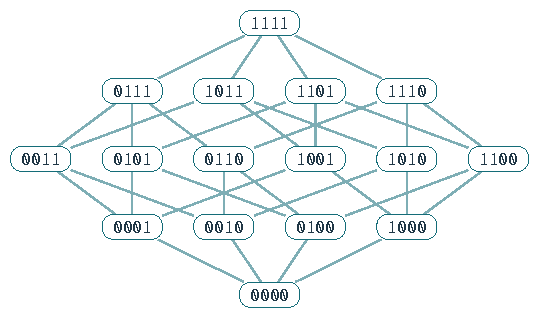
\includegraphics[width=.82\linewidth]{figures/chapter-duality/boolean-cube/figure.pdf}
\caption{The Boolean cube $\FF_2^4$, arranged by Hamming weight. Each edge changes exactly one coordinate.}
\label{fig-cube-booleen}
\end{figure}

\subsection{Characters of the Boolean cube}
\label{sect2-presentation-transforme-walsh}
For $a=(a_0,\ldots,a_{k-1})\in\FF_2^k$, define
\begin{equation}
\label{eq-denf-base-walsh}
 \chi_a(x)=(-1)^{\dotp ax},\qquad
 \dotp ax=\sum_{j=0}^{k-1}a_jx_j\quad\text{in }\FF_2.
\end{equation}
These are exactly the characters of the cube. Identify a binary vector $x$
with the integer $\sum_jx_j2^j$ in $\{0,\ldots,2^k-1\}$. This gives a
\emph{natural order} of both the group elements and their characters.
The identification is a bijection of sets; binary-vector addition corresponds
to bitwise exclusive-or, not integer addition modulo $2^k$.

\begin{exmp}
\label{notation-32}
For $k=3$, the character table is the Walsh matrix
\begin{equation}
\label{eqn-matrix-walsh-8}
 W_8=\begin{pmatrix}
 1&1&1&1&1&1&1&1\\
 1&-1&1&-1&1&-1&1&-1\\
 1&1&-1&-1&1&1&-1&-1\\
 1&-1&-1&1&1&-1&-1&1\\
 1&1&1&1&-1&-1&-1&-1\\
 1&-1&1&-1&-1&1&-1&1\\
 1&1&-1&-1&-1&-1&1&1\\
 1&-1&-1&1&-1&1&1&-1
 \end{pmatrix}.
\end{equation}
Its entry $(i,j)$ is $\chi_i(j)$. Figure~\ref{fig-matrices-walsh} shows
$W_{64}$, with white entries for $1$ and black entries for $-1$.

\begin{figure}[tbp]
\centering
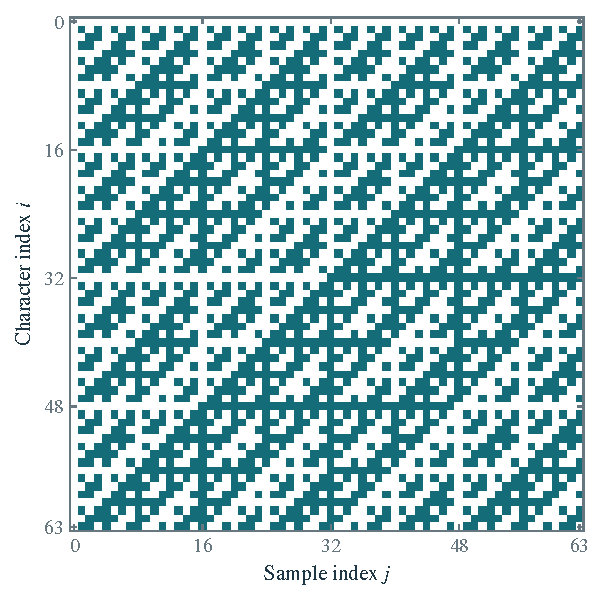
\includegraphics[width=.53\linewidth]{figures/chapter-duality/walsh-matrix/figure.pdf}
\caption{The Walsh matrix $W_{64}$ in natural order. White represents $+1$ and dark teal represents $-1$.}
\label{fig-matrices-walsh}
\end{figure}
\end{exmp}

\begin{defn}[Walsh transform]
\label{notation-33}
For a vector $f\in\CC^{2^k}$, define
\begin{equation}
\label{eq-formula-defn-trans-walsh}
 \Ww_k(f)[i]=\sum_{j=0}^{2^k-1}f[j]\chi_i(j)
 =2^k\dotp f{\chi_i},\qquad 0\leq i<2^k.
\end{equation}
Thus $\Ww_k(f)=W_{2^k}f$.
\end{defn}
Because the characters are real-valued, this is also $\wh f(\chi_i)$ under
the convention of Chapter~1. No conjugation changes the result.

On the cube, the \emph{degree} of a character is the number of nonzero
coordinates in its index $a$: a character of degree $d$ is the product of
$d$ coordinate characters. Small degree is important in Boolean function
analysis. A different ordering, by the number of sign changes along the
integer-indexed row, is called \emph{sequency order}. The two notions should
not be confused; Exercise~\ref{exo-compression-walsh} develops the latter.

\begin{prop}[Inversion]
\label{prop-pte-matrix-hadamard}
The Walsh matrix is real and symmetric and satisfies
$W_{2^k}^2=2^kI$. Consequently,
\[
 \Ww_k^{-1}=2^{-k}\Ww_k,
 \qquad
 f[i]=2^{-k}\sum_{j=0}^{2^k-1}\Ww_k(f)[j]\chi_j(i).
\]
\end{prop}
\begin{proof}
Symmetry follows from $\dotp ij=\dotp ji$. Character orthogonality gives
$W_{2^k}W_{2^k}^{\mathsf T}=2^kI$, which proves the assertions.
\end{proof}

\subsection{A fast algorithm}
\label{sect2-fwt}
\index{Fast Walsh transform}\index{Divide and conquer}
Split $f$ into its first and second halves, $f_1$ and $f_2$, each of length
$2^{k-1}$. Separating the highest binary coordinate in
\eqref{eq-formula-defn-trans-walsh} gives
\[
 \Ww_k(f)=
 \begin{pmatrix}
 \Ww_{k-1}(f_1)+\Ww_{k-1}(f_2)\\
 \Ww_{k-1}(f_1)-\Ww_{k-1}(f_2)
 \end{pmatrix}.
\]
Equivalently,
\[
 W_{2^k}=
 \begin{pmatrix}W_{2^{k-1}}&W_{2^{k-1}}\\
                 W_{2^{k-1}}&-W_{2^{k-1}}\end{pmatrix},\qquad W_1=(1).
\]
This recursion is the \emph{fast Walsh transform} (FWT). For $n=2^k$,
its arithmetic cost satisfies $C(n)=2C(n/2)+n$, with $C(1)=0$.
There are $\log_2n$ levels, each requiring $n$ additions or subtractions,
so $C(n)=n\log_2n$. Program~\ref{listing-fwt} implements the recursion in
Python. Exercise~\ref{exo-tensor-product} explains its tensor-product structure.
The FFT of the next chapter uses the same divide-and-conquer principle.

\subsection{Uses and limitations}
\label{sect2-use-fwt}
The Walsh transform decomposes functions into a simple orthogonal basis and
is particularly convenient for binary data. It supports factorial contrasts
in statistics (Exercise~\ref{exo-transforme-walsh-statistic}), signal
compression (Exercise~\ref{exo-compression-walsh}), and Boolean function
analysis (Exercises~\ref{exo-boolean-functions} and~\ref{exo-learning-boolean-functions}).

As a group Fourier transform, it also satisfies a convolution theorem.
Writing $x\oplus y$ for bitwise exclusive-or, define
\[
 (f*_\oplus g)[x]=\sum_y f[y]g[x\oplus y].
\]
Then $\Ww_k(f*_\oplus g)=\Ww_k(f)\cdot\Ww_k(g)$.
The Walsh transform generally does \emph{not} diagonalize the circular
convolution based on subtraction modulo $2^k$. That operation belongs to
the cyclic group and is diagonalized by the DFT. The distinction is the group
law, not a failure of the convolution theorem.

\section{Poisson summation}
\label{sect1-fish-formula}
Poisson summation relates restriction to a subgroup and restriction of the
Fourier transform to its annihilator. In a vector space over $\FF_2$, this
becomes a statement about orthogonal subspaces and leads to the MacWilliams
identity for weight enumerators.

\subsection{The finite-group formula}
\label{abelian-finite-grpe-fish-formula}
\label{notation-34}\label{notation-35}\label{notation-36}
Recall first the linear-algebraic pairing between a finite-dimensional
$k$-vector space $E$ and its dual $E^*=\Hom_k(E,k)$:
$\dotp x\ell=\ell(x)$. For $A\subset E$, its annihilator is
\begin{equation}
\label{eq-defn-orthogonal-ev}
 A^\perp=\{\ell\in E^*: \ell(x)=0\text{ for every }x\in A\}.
\end{equation}
It is a subspace of $E^*$. Conversely, for $B\subset E^*$,
$B^0=\{x\in E:\ell(x)=0\text{ for every }\ell\in B\}$ is a subspace of $E$.
On subspaces, these operations are inverse, inclusion-reversing bijections.
See Ramis, Deschamps, and Odoux~\cite{ramis-1}.

\begin{defn}[Annihilator of a subgroup]
\label{defn-orthogonal-abelian-subgroup}\label{notation-37}
\index{Annihilator!of a subgroup}
For a subgroup $H$ of a finite abelian group $G$, define
\[
 H^\sharp=\{\chi\in\wh G:\chi(h)=1\text{ for every }h\in H\}.
\]
This subgroup of $\wh G$ is also called the orthogonal of $H$.
\end{defn}
By Lemma~\ref{lem-suite-exact}, pullback from $G/H$ gives a canonical
identification $H^\sharp\simeq\widehat{G/H}$ and
$|H^\sharp|=|G|/|H|$. The operation reverses inclusions, and
$(H^\sharp)^\sharp=H$ after identifying $G$ with its bidual.
Indeed, the double annihilator contains $H$ and has the same order.

\begin{thm}[Finite Poisson summation]
\index{Poisson summation!finite groups}
For $f:G\to\CC$, a subgroup $H\subset G$, and $g\in G$,
\begin{equation}
\label{eq-formula-fish-finished-grp}
 \sum_{h\in H}f(gh)
 =\frac{|H|}{|G|}\sum_{\chi\in H^\sharp}\wh f(\ol\chi)\chi(g).
\end{equation}
\end{thm}
\begin{proof}
Periodize $f$ over $H$ by setting
$\wt f(gH)=\sum_{h\in H}f(gh)$.
Replacing $g$ by $gh_0$, with $h_0\in H$, merely permutes the sum, so this
is a well-defined function on $G/H$.
Its Fourier expansion is
\begin{equation}
\label{eq-demo-formuel-fish-gpe-finite-tmp}
 \wt f(gH)=\sum_{\chi\in\widehat{G/H}}
                c_{\wt f}(\chi)\chi(gH).
\end{equation}
Choose representatives $S$ for $G/H$. Identifying each quotient character
with its pullback, its Fourier coefficient is
\begin{align}
\label{eq-formula-fish-intermediate-result}
 c_{\wt f}(\chi)
 &=\frac1{|G/H|}\sum_{s\in S}\sum_{h\in H}f(sh)\ol{\chi(s)}\nonumber\\
 &=\frac{|H|}{|G|}\sum_{x\in G}f(x)\ol{\chi(x)}
 =\frac{|H|}{|G|}\wh f(\ol\chi).
\end{align}
Here $(s,h)\mapsto sh$ is a bijection $S\times H\to G$, and $\chi(sh)=\chi(s)$.
Substitute in the Fourier expansion and use
$\widehat{G/H}\simeq H^\sharp$.
\end{proof}
At $g=1$, inversion permutes $H^\sharp$, giving the common form
\begin{equation}
\label{eq-formula-fish-group-finite-simple}
 \sum_{h\in H}f(h)=\frac{|H|}{|G|}
                       \sum_{\chi\in H^\sharp}\wh f(\chi).
\end{equation}

There is also a useful proof by comparing the trace of a convolution operator
in two bases. Pullback along $G\to G/H$ identifies $\CC[G/H]$ with the
subspace $V_H\subset\CC[G]$ of functions constant on cosets of $H$.

\begin{proof}[A trace proof]
Let $A_f:u\mapsto f*u$. Translation invariance of convolution implies
$A_f(V_H)\subset V_H$. A basis of $V_H$ consists of the coset indicators
$e_{sH}=\mathbf{1}_{sH}$, for $s\in S$. These are not point masses on $G$.
For each diagonal entry,
\[
 (A_fe_{sH})(s)=\sum_{x\in G}f(x)e_{sH}(x^{-1}s)
 =\sum_{h\in H}f(h).
\]
Consequently,
\[
 \Tr(A_f|_{V_H})=\frac{|G|}{|H|}\sum_{h\in H}f(h).
\]
A second basis of $V_H$ is the character family $H^\sharp$.
The eigenvalue associated with $\chi$ is $\wh f(\chi^{-1})$, as shown in
Exercise~\ref{exo-determinant-circulating}. Thus
\[
 \Tr(A_f|_{V_H})=\sum_{\chi\in H^\sharp}\wh f(\chi^{-1})
 =\sum_{\chi\in H^\sharp}\wh f(\chi).
\]
Comparing the traces proves \eqref{eq-formula-fish-group-finite-simple}.
For the full formula, apply it to $f_g(x)=f(gx)$ and use
$\wh f_g(\chi)=\chi(g)^{-1}\wh f(\chi)$, then reindex by inversion.
\end{proof}

\subsection{The MacWilliams identity}
\label{sect2-application-id-mac-williams}
\index{MacWilliams identity}
Take $G=\FF_2^k$. Every additive subgroup is an $\FF_2$-linear subspace,
because multiplication by either scalar $0$ or $1$ preserves it.
Under the pairing $a\mapsto\chi_a$, we have
\begin{equation}
\label{eq-equivalence-orthogonalite-caractere}
 \chi_a\in H^\sharp
 \quad\Longleftrightarrow\quad
 \dotp ah=0\text{ for every }h\in H
 \quad\Longleftrightarrow\quad a\in H^\perp.
\end{equation}
Thus the group annihilator corresponds to the linear orthogonal.
The dot product over $\FF_2$ is nondegenerate but not positive definite:
for example, $(1,1,1,1)$ is orthogonal to itself. In particular, $H^\perp$
need not be a complementary subspace to $H$.

For extension fields, an additive subgroup need not be a linear subspace
over the whole field. Exercise~\ref{exo-generalization-mac-williams} treats
the generalization with the required linearity assumption.

\begin{prop}[Vector-space Poisson summation]
\label{prop-formula-vector-fish}
For an $\FF_2$-linear subspace $H\subset\FF_2^k$ and a function
$f:\FF_2^k\to\CC$,
\begin{align}
\label{eq-formula-fish-vector-1}
 \sum_{a\in H}f(a)&=\frac{|H|}{2^k}
                         \sum_{u\in H^\perp}\wh f(\chi_u),\\
\label{eq-formula-vector-fish-2}
 \sum_{a\in H^\perp}f(a)&=\frac1{|H|}
                         \sum_{u\in H}\wh f(\chi_u).
\end{align}
\end{prop}
\begin{proof}
The first identity is finite Poisson summation under
\eqref{eq-equivalence-orthogonalite-caractere}.
For the second, replace $H$ by $H^\perp$, using
$|H^\perp|=2^k/|H|$ and $(H^\perp)^\perp=H$.
\end{proof}

\begin{defn}[Hamming weight and distance]
\label{notation-38}\label{notation-39}\index{Hamming distance}
For $z\in\FF_2^k$, its weight is the number of nonzero coordinates,
$w(z)=|\{i:z_i\neq0\}|$. The Hamming distance is
\[
 d(x,y)=w(x-y)=|\{i:x_i\neq y_i\}|.
\]
In characteristic two, $x-y=x+y$.
\end{defn}
In Figure~\ref{fig-cube-booleen}, edges join vectors at Hamming distance one.
To record the distribution of weights in a subspace, introduce a polynomial.

\begin{defn}[Weight enumerator]
\label{notation-40}\index{Weight enumerator}
For $H\subset\FF_2^k$, define
\[
 A_H(X,Y)=\sum_{c\in H}X^{k-w(c)}Y^{w(c)}
 =\sum_{i=0}^k A_iX^{k-i}Y^i,
\]
where $A_i$ is the number of vectors in $H$ of weight $i$.
\end{defn}

\begin{thm}[MacWilliams identity]
\label{thm-id-mac-williams}
For a linear subspace $H\subset\FF_2^k$,
\[
 A_{H^\perp}(X,Y)=\frac1{|H|}A_H(X+Y,X-Y).
\]
\end{thm}
\begin{proof}
Fix $x,y\in\CC$ and set $f(t)=x^{k-w(t)}y^{w(t)}$.
The Walsh transform factors coordinate by coordinate:
\begin{align*}
 \wh f(\chi_a)
 &=\sum_{t\in\FF_2^k}\prod_{j=0}^{k-1}
              x^{1-t_j}y^{t_j}(-1)^{a_jt_j}\\
 &=\prod_{j=0}^{k-1}\left(x+(-1)^{a_j}y\right)
 =(x+y)^{k-w(a)}(x-y)^{w(a)}.
\end{align*}
Insert this expression in \eqref{eq-formula-vector-fish-2}.
The equality holds for every $(x,y)\in\CC^2$, so it is a polynomial identity.
\end{proof}
This relates the entire weight distribution of a linear code to that of its
dual. Section~\ref{sect1-codes-correctors-duality} develops its coding-theoretic
consequences.

\subsection{Continuous Poisson summation}
\index{Poisson summation!continuous}
For this subsection, use the frequency convention
\begin{equation}
\label{eq-defn-trans-fourier-special-fish}
 \wh f(\xi)=\int_{\RR}f(t)e^{-2\pi\imath t\xi}\,\d t.
\end{equation}
The finite-group proof extends by periodization, provided we justify
convergence and the interchange of sums and integrals.

\begin{thm}[Continuous Poisson summation]
\label{thm-formula-fish-continue}
Let $f:\RR\to\CC$ be continuous and suppose that
\begin{align}
\label{eq-formula-fish-hyp1}
 |f(x)|&\leq M(1+|x|)^{-\alpha}
          \quad\text{for some }M>0,\ \alpha>1,\\
\label{eq-formula-fish-hyp2}
 \sum_{n\in\ZZ}|\wh f(n)|&<\infty.
\end{align}
Then
\begin{equation}
\label{eq-formula-fish-continue}
 \sum_{n\in\ZZ}f(n)=\sum_{n\in\ZZ}\wh f(n).
\end{equation}
\end{thm}
\begin{proof}
Define $f_1(x)=\sum_{n\in\ZZ}f(x+n)$.
For $|x|\leq A$ and $|n|\geq2A$,
\[
 |f(x+n)|\leq M(1+|n|-A)^{-\alpha}
             \leq M(1+|n|/2)^{-\alpha}.
\]
The last bound is summable. Hence the periodization converges uniformly on
compact intervals, is continuous, and is $1$-periodic.
Its Fourier coefficient at $m\in\ZZ$ is
\begin{align*}
 c_m(f_1)
 &=\int_0^1\sum_{n\in\ZZ}f(t+n)e^{-2\pi\imath mt}\,\d t\\
 &=\sum_{n\in\ZZ}\int_n^{n+1}f(u)e^{-2\pi\imath mu}\,\d u
 =\wh f(m).
\end{align*}
Uniform convergence justifies the first interchange, and $f\in L^1(\RR)$
justifies the sum over intervals. The second hypothesis makes
$\sum_m\wh f(m)e^{2\pi\imath mx}$ uniformly convergent. Its sum and $f_1$
have identical Fourier coefficients; uniqueness and continuity imply
\[
 \sum_{n\in\ZZ}f(x+n)=\sum_{m\in\ZZ}\wh f(m)e^{2\pi\imath mx}.
\]
Set $x=0$.
\end{proof}

\begin{rem}[The quotient viewpoint]
Here the subgroup is $\ZZ\subset\RR$, and periodization produces a function
on $\RR/\ZZ$. Its characters are $x\mapsto e^{2\pi\imath mx}$, indexed by
$m\in\ZZ$. Thus the same quotient-and-dual construction underlies the
finite and continuous formulas. In the continuous setting the constants
are determined by the chosen Haar measures and Fourier convention.
\end{rem}

\begin{defn}[Jacobi's theta function]
\index{Theta function}
For $t>0$, define
\[
 \theta(t)=\sum_{n\in\ZZ}e^{-\pi n^2t}.
\]
\end{defn}

\begin{lem}[Fourier transform of a Gaussian]
\label{lem-tf-gaussienne}
For $t>0$, let $g_t(x)=e^{-x^2/(2t)}$. Under
\eqref{eq-defn-trans-fourier-special-fish},
\[
 \wh g_t(\xi)=\sqrt{2\pi t}\,e^{-2\pi^2t\xi^2}.
\]
\end{lem}
\begin{proof}
Differentiation under the integral is justified by the integrability of
$|x|g_t(x)$. Since $xg_t(x)=-tg_t'(x)$, integration by parts gives
\[
 \frac{\d}{\d\xi}\wh g_t(\xi)=-4\pi^2t\xi\wh g_t(\xi).
\]
The boundary term vanishes by Gaussian decay. Solving this differential
equation gives $\wh g_t(\xi)=\wh g_t(0)e^{-2\pi^2t\xi^2}$.
The substitution $x=\sqrt t\,u$ gives $\wh g_t(0)=\sqrt t\,I$, where
$I=\int_\RR e^{-u^2/2}\,\d u$. Tonelli's theorem and polar coordinates yield
\[
 I^2=\int_{\RR^2}e^{-(u^2+v^2)/2}\,\d u\,\d v
 =2\pi\int_0^\infty re^{-r^2/2}\,\d r=2\pi.
\]
Since $I>0$, the constant is $\sqrt{2\pi t}$.
\end{proof}

\begin{thm}[Jacobi's identity]
\begin{equation}
\label{eq-id-jacobi}
 \theta(t)=\frac1{\sqrt t}\theta(1/t),\qquad t>0.
\end{equation}
\end{thm}
\begin{proof}
Apply Poisson summation to $h_t(x)=e^{-\pi t x^2}=g_{1/(2\pi t)}(x)$.
The preceding lemma gives
$\wh h_t(\xi)=t^{-1/2}e^{-\pi\xi^2/t}$, and both decay hypotheses hold.
\end{proof}
For small $t$, this identity greatly accelerates evaluation. On the right,
keeping only the term $n=0$ approximates $\theta(t)$ by $t^{-1/2}$, with
relative error bounded by
\[
 0<\frac{\theta(t)-t^{-1/2}}{t^{-1/2}}
 =2\sum_{n=1}^{\infty}e^{-\pi n^2/t}
 \leq\frac{2e^{-\pi/t}}{1-e^{-3\pi/t}}.
\]
For $t=0.001$ this truncation error is far below double-precision rounding.
The computed value is still subject to floating-point rounding; the identity
reduces the number of terms, not the machine's rounding error.

\section{Exercises}

\begin{exo}[A geometric proof of quadratic reciprocity]
\label{exo-proof-geom-reciprocite}
Let $p$ and $r$ be distinct odd primes, and let $[x]_p\in\{0,\ldots,p-1\}$
denote the least nonnegative residue of an integer $x$ modulo $p$.
We will prove \eqref{eq-reciprocity-quadratic} by counting lattice points.
\begin{enumerate}
\item Set $E=\{2,4,\ldots,p-1\}$ and $B_r=\{[ra]_p:a\in E\}$.
Prove that $E=\{[(-1)^bb]_p:b\in B_r\}$.
\item Multiply the elements in these sets and use Euler's criterion to obtain
\[
 \legsymb rp=(-1)^{\sum_{b\in B_r}b}.
\]
\item Use Euclidean division of $ra$ by $p$ to prove
\[
 \sum_{a\in E}ra=p\sum_{a\in E}\left\lfloor\frac{ra}{p}\right\rfloor
                  +\sum_{b\in B_r}b,
 \qquad
 \legsymb rp=(-1)^{\sum_{a\in E}\lfloor ra/p\rfloor}.
\]
\item In Figure~\ref{fig-demo-geom-reciprocite}, let
$A=(0,0)$, $D=(p,0)$, $B=(p,r)$, $K=(p/2,0)$,
$L=(0,r/2)$, and $H=(p/2,r/2)$.
Show that the open diagonal segment $AB$ contains no lattice point.
Interpret $t_a=\lfloor ra/p\rfloor$ as the number of lattice points with
abscissa $a$ strictly between the horizontal axis and $AB$.
\item Show that $t_{p-a}=r-1-t_a$, so $t_{p-a}\equiv t_a\pmod2$.
Each pair $\{a,p-a\}$ contains exactly one even integer. Deduce that
\[
 \sum_{a\in E}t_a\equiv\sum_{a=1}^{(p-1)/2}t_a\pmod2.
\]
Interpret the right-hand side as the number of lattice points strictly
inside the triangle $AKH$.
\item Interchange $p$ and $r$. The two resulting triangles partition the
lattice points strictly inside $AKHL$. Deduce quadratic reciprocity.
\end{enumerate}
\begin{figure}[tbp]
\centering
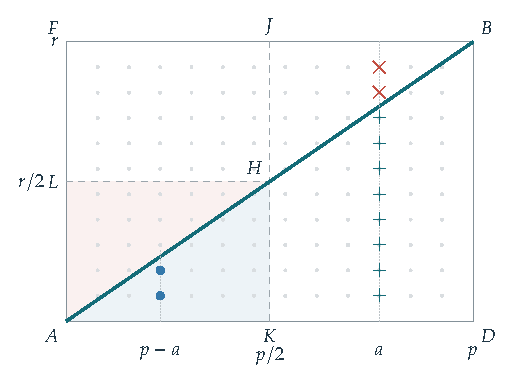
\includegraphics[width=.74\linewidth]{figures/chapter-duality/geometric-reciprocity/figure.pdf}
\caption{Lattice-point pairing in the geometric proof of quadratic reciprocity, illustrated with $p=13$, $r=11$, and $a=10$.}
\label{fig-demo-geom-reciprocite}
\end{figure}
\end{exo}

\begin{exo}[Fermat's equation over a finite field]
\label{exo-thm-fermat-finite-body}\index{Fermat's equation}
Let $q$ be a prime power and $k\geq1$ an integer. Using the counting estimates
of Exercise~\ref{exo-eqn-grpe-abelien-finite}, prove that $q\geq k^4+4$
guarantees a solution of
\begin{equation}
\label{eq-thm-fermat-finite-body}
 x^k+y^k=z^k,\qquad x,y,z\in\FF_q^*.
\end{equation}
All Fourier transforms in this exercise are on the additive group of $\FF_q$.
\begin{enumerate}
\item Suppose first that $k\mid q-1$. Show that the unique multiplicative
subgroup of index $k$ is $H_k=\{x^k:x\in\FF_q^*\}$.
\item Let $\chi_0,\ldots,\chi_{k-1}$ be the characters of
$\FF_q^*/H_k$, pulled back to $\FF_q^*$. Show that for every additive
character $\psi$,
\[
 \wh{f_{H_k}}(\psi)=\frac1k\sum_{i=0}^{k-1}G(\chi_i,\psi).
\]
Deduce from the Gauss-sum estimates that $\Phi(H_k)<\sqrt q$, where
$\Phi$ is defined in \eqref{eq-defn-phi-ensemble}.
\item For nonempty subsets $A_1,A_2\subset\FF_q^*$, let $N$ and $N'$
count, respectively, the solutions of
\begin{align}
\label{eq-thm-fermat_intermediaire}
 x+y&=z^k,& x\in A_1,\quad y\in A_2,\quad z\in\FF_q^*,\\
 x+y&=u,& x\in A_1,\quad y\in A_2,\quad u\in H_k.\nonumber
\end{align}
Show that $N=kN'$ and, by applying the counting estimate to
$A_1,A_2,-H_k$, prove
\begin{equation}
\label{eqn-fermat-majoration}
 \left|N-\frac{|A_1||A_2|(q-1)}q\right|
       <k\sqrt{|A_1||A_2|q}.
\end{equation}
\item Write $l_i=(q-1)/|A_i|$. Prove that $q\geq k^2l_1l_2+4$ implies
$N>0$. For general $k$, show that the sets of nonzero $k$th powers and
$d$th powers coincide, where $d=\gcd(k,q-1)$, and extend the criterion.
\item Apply it with $A_1=A_2=H_d$ to prove the claimed sufficient condition
for \eqref{eq-thm-fermat-finite-body}.
\end{enumerate}
\end{exo}

\begin{exo}[Walsh transforms and factorial contrasts]
\label{exo-transforme-walsh-statistic}
This example, adapted from Maslen and Rockmore~\cite{rockmore-generalized},
illustrates Yates's algorithm for a two-level factorial experiment.
A farmer measures wheat height under three factors: lighting $a$, herbicide
$b$, and fertilizer $c$. Each factor is set high ($+$) or low ($-$).
The observed heights, in centimeters, are
\[
\begin{array}{ccc|r@{\qquad}ccc|r}
 a&b&c&\alpha_{abc}&a&b&c&\alpha_{abc}\\\hline
 +&+&+&69&+&+&-&61\\
 -&+&+&81&-&+&-&92\\
 +&-&+&63&+&-&-&54\\
 -&-&+&77&-&-&-&89
\end{array}
\]
Encode $+$ by $0$ and $-$ by $1$, with $a$ the least significant bit.
The data vector is therefore $f=(69,81,63,77,61,92,54,89)$.
The grand mean is $\mu=\frac18\sum\alpha_{abc}$. For a nonempty subset
$S\subset\{a,b,c\}$, define its factorial effect by
\[
 \mu_S=\frac14\sum_{(a,b,c)\in\{+1,-1\}^3}
                   \alpha_{abc}\prod_{s\in S}s.
\]
For instance, $\mu_a$ is the mean at high lighting minus the mean at low
lighting, averaged over the other two factors. Higher-order contrasts measure
interactions under the same normalization. Express all seven effects and the
mean using a single Walsh transform, and compute them for the given data.
These contrasts describe the observations; assessing statistical significance
would also require a model for experimental variability.
\end{exo}

\begin{exo}[The Haar basis and its fast transform]
\label{exo-wavelet-haar}\index{Wavelet!Haar}\index{Basis!Haar}
Let $\psi_0=\mathbf1_{[0,1)}$ and
$\psi=\mathbf1_{[0,1/2)}-\mathbf1_{[1/2,1)}$. Define
\[
 \psi_{j,k}(x)=2^{j/2}\psi(2^jx-k),\qquad
 j\geq0,\quad 0\leq k<2^j,
 \qquad \psi_n=\psi_{j,k}\quad\text{when }n=2^j+k.
\]
Let $F_J$ be the space of functions constant on each dyadic interval
$[k2^{-J},(k+1)2^{-J})$, for $0\leq k<2^J$.
All inner products in this exercise are the usual integral inner product on
$L^2([0,1])$. For pointwise statements on $[0,1]$, assign each step function
its left limit at $1$.
\begin{enumerate}
\item Prove that $\psi_0,\ldots,\psi_{2^J-1}$ form an orthonormal basis
of $F_J$.
\item For $f\in C([0,1])$, its orthogonal projection onto $F_J$ is
\[
 f_J=\dotp f{\psi_0}\psi_0+
       \sum_{j=0}^{J-1}\sum_{k=0}^{2^j-1}\dotp f{\psi_{j,k}}\psi_{j,k}.
\]
Show that it is the average of $f$ on each dyadic interval and converges
uniformly to $f$. Prove the same convergence for every partial sum
$\wt f_n=\sum_{m=0}^n\dotp f{\psi_m}\psi_m$.
Hint: a partial sum within one wavelet level averages $f$ on a partition
in which only some of the dyadic intervals have been bisected.
Deduce that the Haar family is a complete orthonormal basis of $L^2([0,1])$.
\begin{figure}[tbp]
\centering
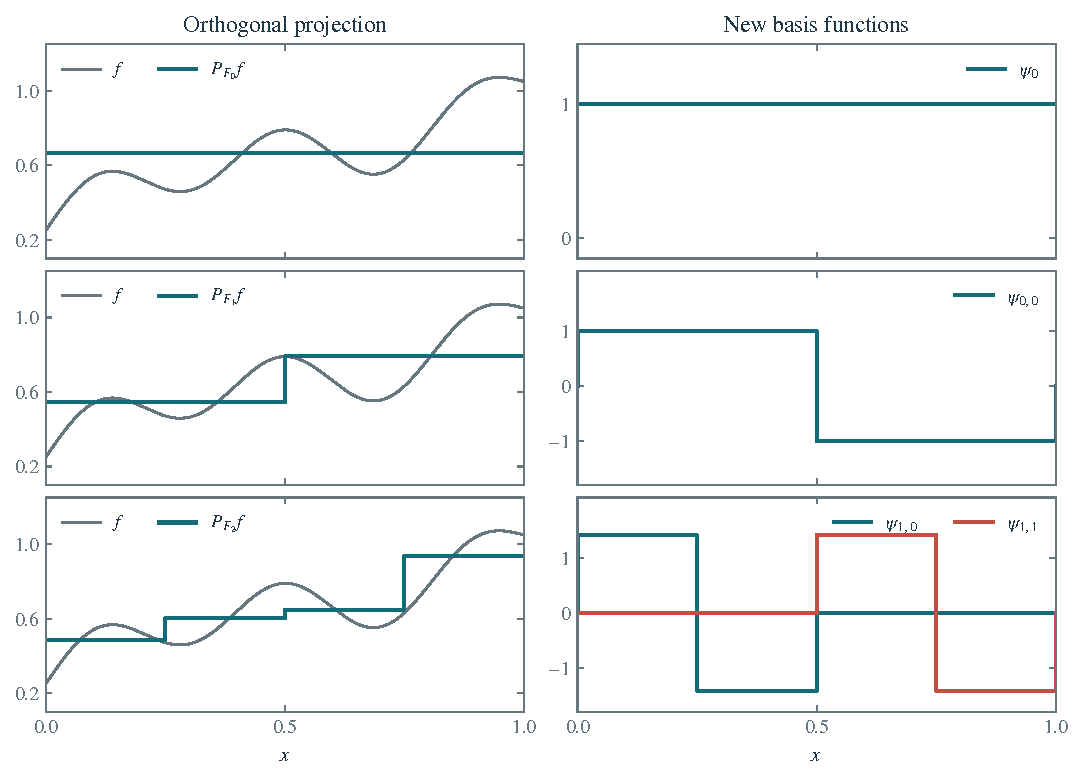
\includegraphics[width=1.0\linewidth]{figures/chapter-duality/haar-projections/figure.pdf}
\caption{Successive Haar projections onto $F_0$, $F_1$, and $F_2$ (left), and the orthonormal basis functions added at each stage (right).}
\label{fig-decomposition-base-haar}
\end{figure}
\item Define $\varphi_{j,k}(x)=2^{j/2}\psi_0(2^jx-k)$.
Show that these functions form an orthonormal basis of $F_j$, and that
\[
 F_{j+1}=F_j\mathbin{\overset{\perp}{\oplus}}G_j,
 \qquad G_j=\operatorname{span}\{\psi_{j,k}:0\leq k<2^j\}.
\]
Express $\varphi_{j,k}$ and $\psi_{j,k}$ using
$\varphi_{j+1,2k}$ and $\varphi_{j+1,2k+1}$.
\item Let $f\in F_J$ and set $x^{(0)}[k]=\dotp f{\varphi_{J,k}}$.
Relate these coefficients to the values of $f$ on its dyadic cells.
For $i=1,\ldots,J$, define vectors of length $2^{J-i}$ by
\[
 x^{(i)}[k]=\frac{x^{(i-1)}[2k]+x^{(i-1)}[2k+1]}{\sqrt2},
 \qquad
 d^{(i)}[k]=\frac{x^{(i-1)}[2k]-x^{(i-1)}[2k+1]}{\sqrt2}.
\]
Show that each stage is an orthogonal transformation. Is its elementary
$2\times2$ block a rotation? Prove that
$x^{(J)}[0]=2^{J/2}\operatorname{mean}(x^{(0)})$.
\begin{figure}[tbp]
\centering
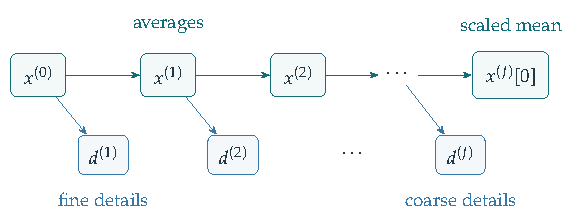
\includegraphics[width=.95\linewidth]{figures/chapter-duality/haar-cascade/figure.pdf}
\caption{The Haar cascade: each stage separates scaling coefficients from details, which are stored from fine to coarse.}
\label{fig-decomposition-wavelet-haar}
\end{figure}
\item Prove that $x^{(i)}[k]=\dotp f{\varphi_{J-i,k}}$ and
$d^{(i)}[k]=\dotp f{\psi_{J-i,k}}$. In particular,
$x^{(J)}[0]=\dotp f{\psi_0}$. Estimate the arithmetic cost of all stages.
\item For $N=2^J$, let $\Gamma$ map the input vector to the concatenation
$(d^{(1)},d^{(2)},\ldots,d^{(J)},x^{(J)})$.
Show that $\Gamma$ is orthogonal and identify the basis vectors whose
coefficients it computes. Compare their supports, and the cost of the
transform, with those of the Walsh basis.
\end{enumerate}
Figure~\ref{fig-transforme-haar} uses this fine-to-coarse packing.
For a smooth signal, neighboring fine-scale values differ little, so their
Haar detail coefficients are small. The last coefficient records the mean
with the orthonormal scaling specified above.
\begin{figure}[tbp]
\centering
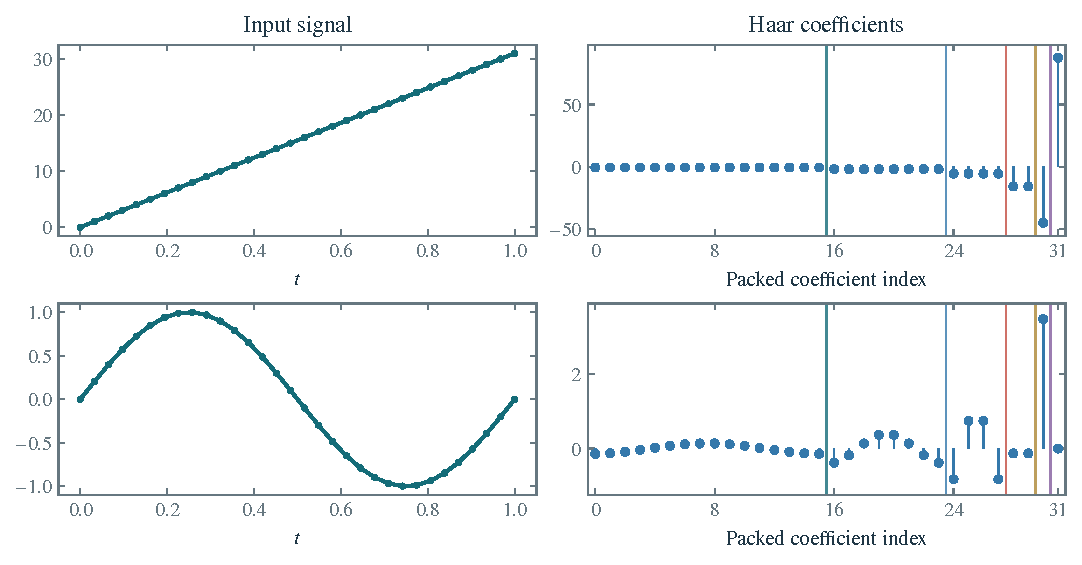
\includegraphics[width=1.0\linewidth]{figures/chapter-duality/haar-examples/figure.pdf}
\caption{Two length-$32$ signals and their orthonormal Haar coefficients. Colored separators mark the detail scales; the final coefficient is the scaled mean.}
\label{fig-transforme-haar}
\end{figure}
Haar analysis is the simplest example of the multiresolution filter-bank
construction developed by Mallat~\cite{mallat}. See also
Exercise~\ref{exo-wavelets-finite-fields} for wavelets over finite fields.
\end{exo}

\begin{exo}[Compression with Walsh functions]
\label{exo-compression-walsh}\index{Compression}\index{Walsh transform!sequency}
The purpose of this exercise is to order the Walsh basis so that initial
segments provide useful approximations to signals and images.
\begin{enumerate}
\item For $N=2^k$, define the two-dimensional basis functions
$\chi_{i,j}(s,t)=\chi_i(s)\chi_j(t)$, for $0\leq i,j,s,t<N$.
Give the forward and inverse transforms, and implement the forward transform
by successive one-dimensional transforms along the two axes.
\item The \emph{sequency} of a Walsh row is the number of sign changes
between consecutive entries, without wrapping the last entry to the first.
Show that the sequencies are precisely $0,1,\ldots,N-1$.
Compare natural and sequency ordering in Figure~\ref{fig-functions-walsh}.
\begin{figure}[tbp]
\centering
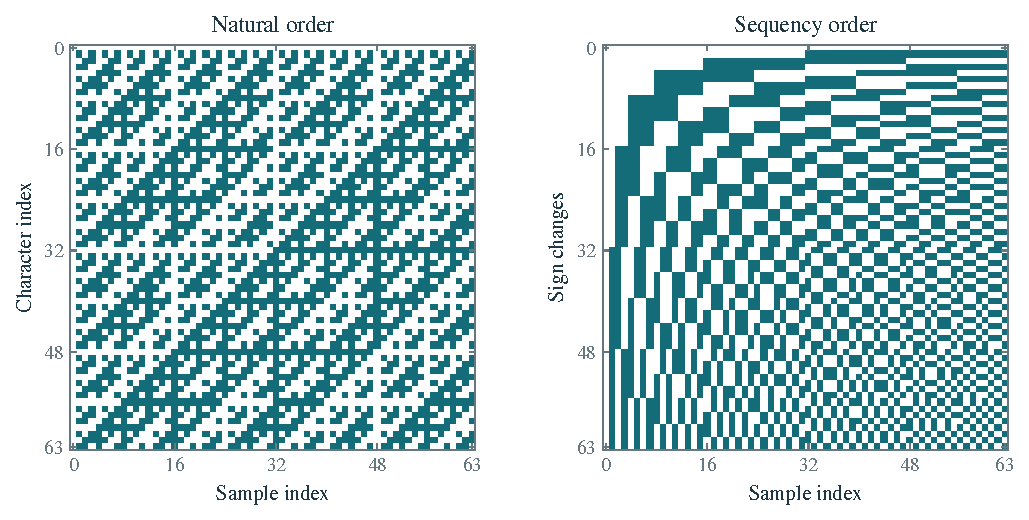
\includegraphics[width=1.0\linewidth]{figures/chapter-duality/walsh-orderings/figure.pdf}
\caption{Walsh functions in natural order and in increasing sequency, with one basis function per row.}
\label{fig-functions-walsh}
\end{figure}
\item Compare the spectra of a smooth signal in these two orders.
Explain in what sense small sequency corresponds to slowly varying functions,
and why it differs from small Hamming degree on the Boolean cube.
\begin{figure}[tbp]
\centering
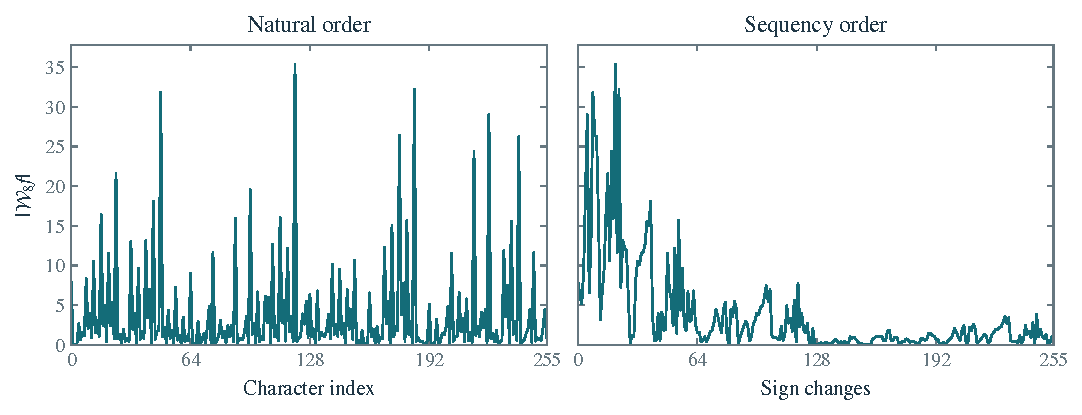
\includegraphics[width=1.0\linewidth]{figures/chapter-duality/walsh-spectrum/figure.pdf}
\caption{The Walsh spectrum of the oscillatory signal in Figure~\ref{fig-compression-walsh-1d}, in natural and sequency order.}
\label{fig-spectrum-walsh-1d}
\end{figure}
\item Write $i_0,\ldots,i_{N-1}$ for the indices in increasing sequency.
For $0\leq M\leq N$, define
\[
 f_M=\sum_{m=0}^{M-1}\dotp f{\chi_{i_m}}\chi_{i_m}
     =\frac1N\sum_{m=0}^{M-1}\Ww_k(f)[i_m]\chi_{i_m},
\]
with the normalized discrete inner product. Explain how storing these $M$
coefficients gives a linear approximation scheme and why their quantization
is also needed for a finite bit representation.
Compare it with low-frequency DFT approximation after reading
Chapter~\ref{chap-tfd}.
\begin{figure}[tbp]
\centering
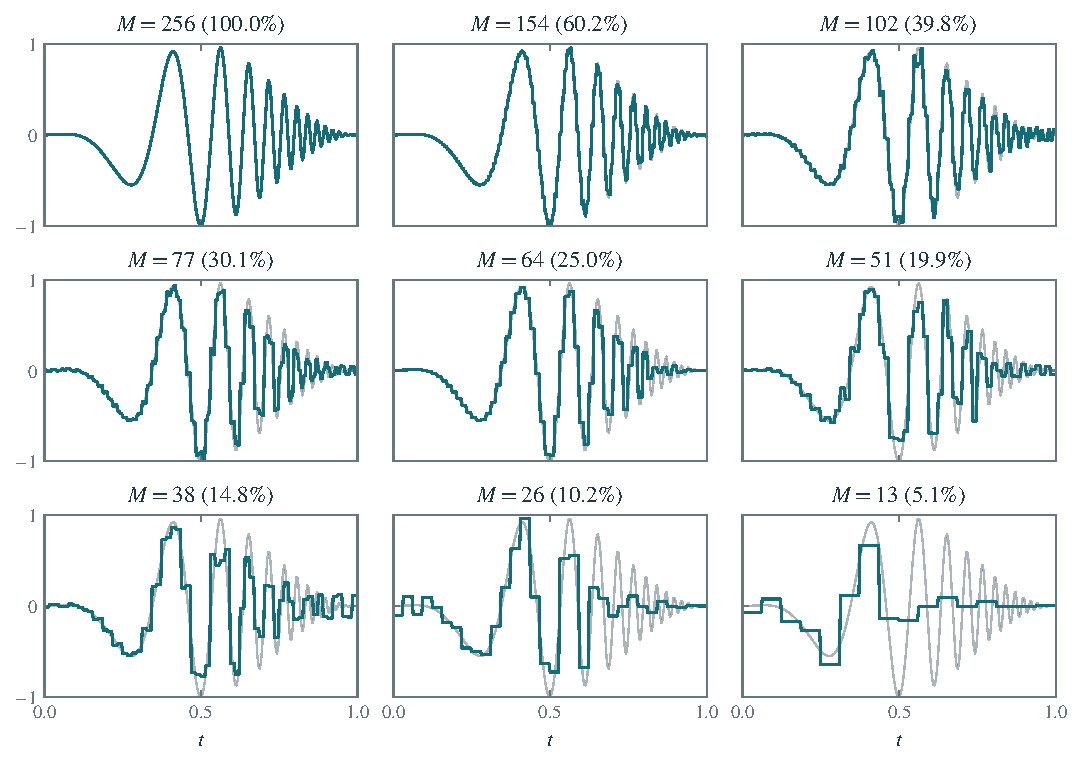
\includegraphics[width=1.0\linewidth]{figures/chapter-duality/walsh-signal-approximation/figure.pdf}
\caption{Progressive approximation of a signal by initial segments of the sequency-ordered Walsh basis. Each panel gives the exact retained coefficient count.}
\label{fig-compression-walsh-1d}
\end{figure}
\item For the two-dimensional functions, suggest an order based on their
horizontal and vertical sequencies. One choice is increasing sum of the two
sequencies, with ties broken by the vertical sequency.
Implement the corresponding image approximation in Python.
\begin{figure}[tbp]
\centering
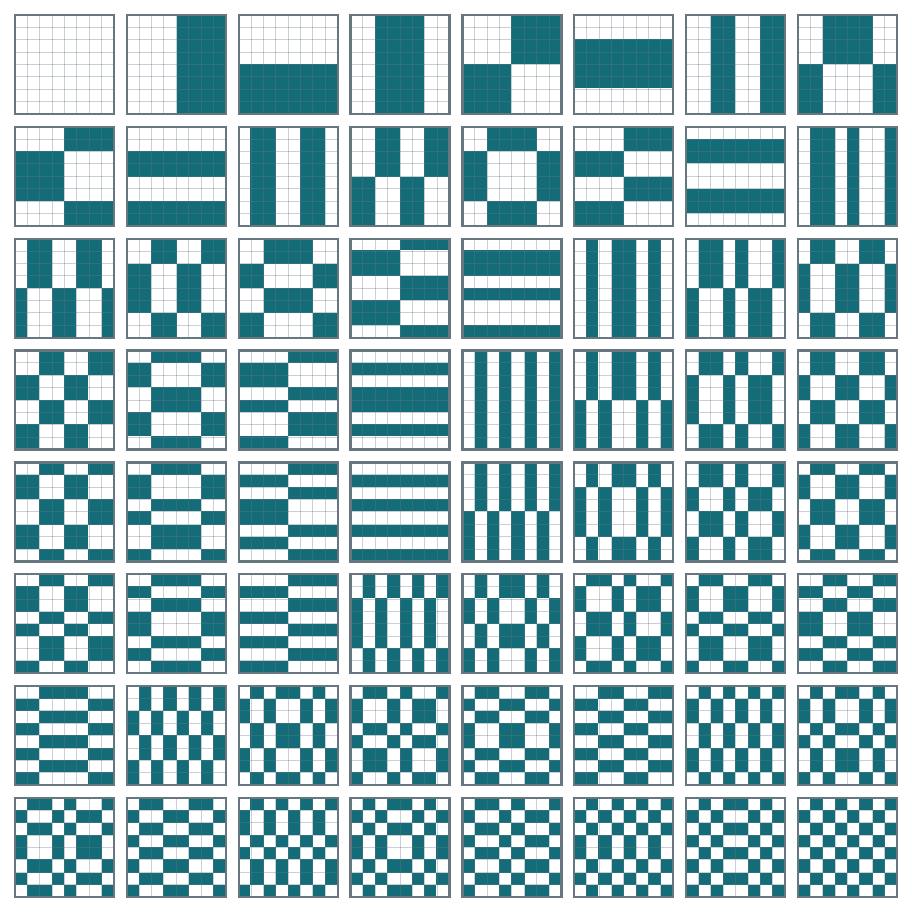
\includegraphics[width=.90\linewidth]{figures/chapter-duality/walsh-basis-two-dimensions/figure.pdf}
\caption{The $64$ two-dimensional Walsh functions for $8\times8$ images, ordered by total sequency and then vertical sequency, from left to right and top to bottom.}
\label{fig-functions-walsh-2d}
\end{figure}
\begin{figure}[tbp]
\centering
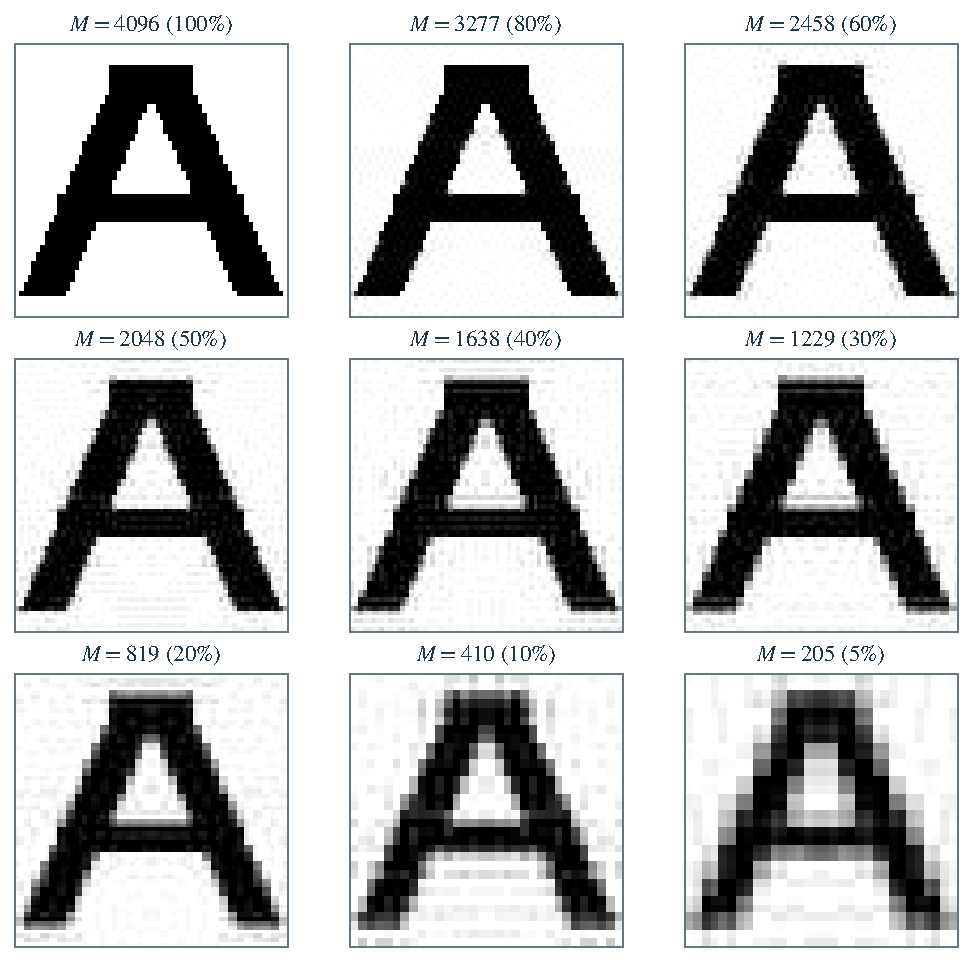
\includegraphics[width=1.0\linewidth]{figures/chapter-duality/walsh-image-approximation/figure.pdf}
\caption{Walsh approximations of a synthetic letter A, with exact retained coefficient counts. Every panel uses the same grayscale range.}
\label{fig-compression-walsh-2d}
\end{figure}
\end{enumerate}
\end{exo}

\begin{exo}[Hadamard matrices]
\label{exo-matrices-hadamard}\index{Hadamard matrix}\index{Paley matrix}
A real $N\times N$ matrix $H_N$ with entries in $\{1,-1\}$ is a
\emph{Hadamard matrix} if $H_NH_N^{\mathsf T}=NI_N$.
\begin{enumerate}
\item Show that the Walsh matrix $W_{2^k}$ is a Hadamard matrix.
\item Show that changing the sign of a row or column, or permuting rows or
columns, preserves this property. Normalize the first row and column to $1$.
If $N\geq3$, group the columns by the four sign patterns of rows two and
three. If their multiplicities are $i,j,k,l$, prove that
$i=j=k=l=N/4$. Thus a Hadamard order is $1$, $2$, or a multiple of $4$.
\item For a prime $p\equiv3\pmod4$, extend the quadratic character by
$\eta(0)=0$ and define
\[
 Q_{ij}=\eta(j-i),\qquad 0\leq i,j<p.
\]
Prove that $Q^{\mathsf T}=-Q$, $QQ^{\mathsf T}=pI_p-J$, and $QJ=JQ=0$,
where $J$ has every entry equal to one.
\item With $\mathbf1\in\RR^p$ a column vector of ones, prove that the
Paley construction
\[
 H_{p+1}=\begin{pmatrix}1&\mathbf1^{\mathsf T}\\
                         \mathbf1&Q-I_p\end{pmatrix}
\]
is a Hadamard matrix. Compute it for $p=7$ and check its Gram matrix.
This supplies a different construction from the tensor powers of $W_2$.
\item If $A\in\RR^{N\times N}$ and $|a_{ij}|\leq1$, prove
\begin{equation}
\label{eq-borne-hadamard}
 |\det A|\leq N^{N/2}.
\end{equation}
Show that a Hadamard matrix attains equality. Also show that a maximizer of
$|\det A|$ on the cube of all such matrices can be chosen with every entry
in $\{1,-1\}$, even when the bound is not attained.
\end{enumerate}
The determinant is the volume of the parallelepiped spanned by the columns.
Its volume is at most the product of their lengths. At a Hadamard matrix,
the columns are mutually orthogonal cube diagonals, each of length $\sqrt N$.
The condition on the order is necessary; the constructions above establish
existence for particular families of orders.
Exercise~\ref{exo-codes-hadamard} applies these matrices to error-correcting codes.
\end{exo}

\begin{exo}[Tensor products of matrices]
\label{exo-tensor-product}\index{Tensor product}
For $A\in\CC^{s\times s}$ and $B\in\CC^{t\times t}$, their tensor product
is the $st\times st$ block matrix
\[
 A\otimes B=(a_{ij}B)_{1\leq i,j\leq s}.
\]
\begin{enumerate}
\item If $AA^*=sI_s$, prove that the tensor power with $n$ factors satisfies
$A^{\otimes n}(A^{\otimes n})^*=s^nI_{s^n}$.
\item Express $W_{2^n}$ as a tensor power.
\item Generalize the FWT recursion to compute $y=A^{\otimes n}x$ without
forming the full matrix. Give the inverse transform and its arithmetic cost
when the base size $s$ is fixed.
\item For
\[
 A_\alpha=\sqrt2\begin{pmatrix}\cos\alpha&\sin\alpha\\
                                  \sin\alpha&-\cos\alpha\end{pmatrix},
\]
show that $U_\alpha=2^{-n/2}A_\alpha^{\otimes n}$ is orthogonal.
Identify its actions at $\alpha=0,\pi/4,\pi/2$.
In particular, distinguish bitwise complementation from reversal of the
\emph{order} of the bits within an index.
\end{enumerate}
Figure~\ref{fig-transfo-walsh-interm} shows the normalized transforms of a
triangular signal. At $\alpha=\pi/4$ the transform is Walsh; at $\pi/2$
it reverses the order of the signal entries, sending index $j$ to $2^n-1-j$.
\begin{figure}[tbp]
\centering
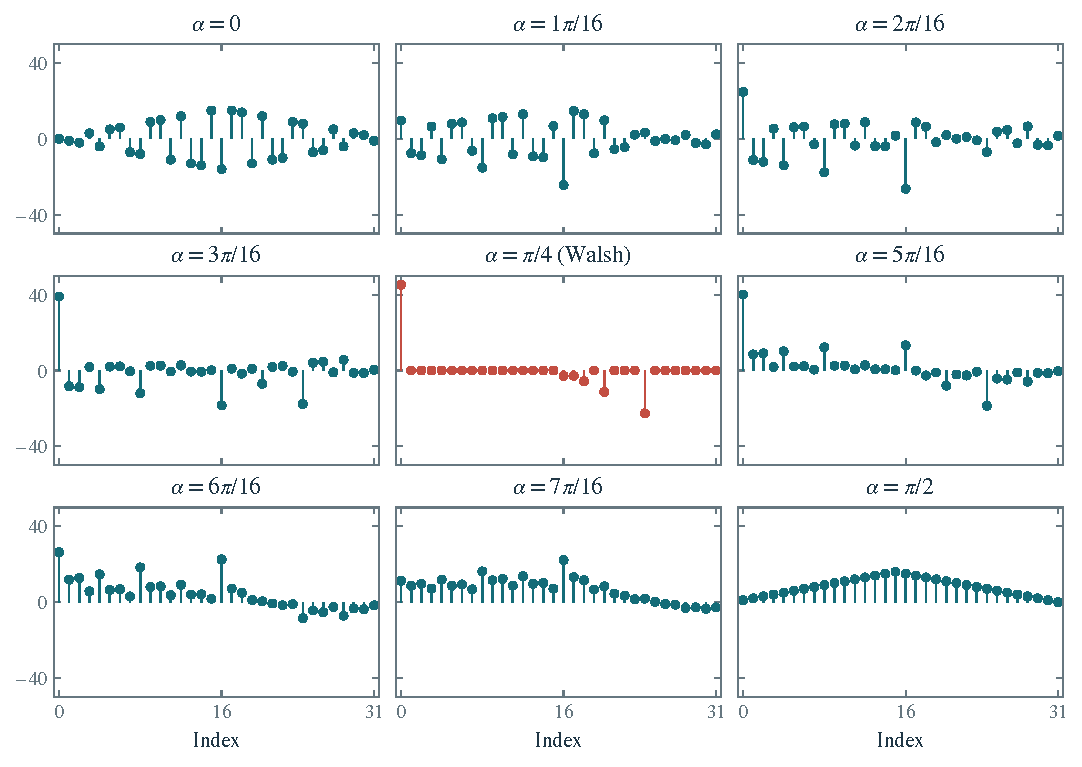
\includegraphics[width=1.0\linewidth]{figures/chapter-duality/intermediate-walsh-transform/figure.pdf}
\caption{Normalized tensor transforms $2^{-n/2}A_\alpha^{\otimes n}$ of a triangular signal, with $n=5$. The middle panel is the Walsh transform; the last reverses the input entries.}
\label{fig-transfo-walsh-interm}
\end{figure}
Exercise~\ref{exo-grpe-quaternionique} constructs another possible base matrix
using representation theory.
\end{exo}

\begin{exo}[The MacWilliams identity over a finite field]
\label{exo-generalization-mac-williams}\index{MacWilliams identity}
Let $q=p^r$ be a prime power, and set $E=\FF_q^k$.
\begin{enumerate}
\item Show that the bilinear form
$\dotp ax=\sum_{i=0}^{k-1}a_ix_i$ is nondegenerate and identifies $E$ with
its $\FF_q$-linear dual.
\item Let $\psi_1$ be the canonical additive character of $\FF_q$
(Definition~\ref{defn-character-additive-canonical}).
For $a\in E$, set $\chi_a(x)=\psi_1(\dotp ax)$.
Use the nondegeneracy of the trace pairing to show that $a\mapsto\chi_a$
is an isomorphism from the additive group $E$ to its character group.
\item Assume that $H\subset E$ is an $\FF_q$-linear subspace.
Prove that its additive annihilator corresponds to its linear orthogonal
$H^\perp$. Explain precisely where closure under multiplication by all
scalars in $\FF_q$ is needed. Give an additive subgroup of $\FF_4$ that
is not an $\FF_4$-linear subspace.
\item With $w(c)$ the number of nonzero coordinates and
$A_H(X,Y)=\sum_{c\in H}X^{k-w(c)}Y^{w(c)}$, prove
\[
 A_{H^\perp}(X,Y)=\frac1{|H|}A_H\bigl(X+(q-1)Y,X-Y\bigr).
\]
\end{enumerate}
\end{exo}

\begin{exo}[Poisson summation for distributions]
\label{exo-formula-fish-distrib}\label{notation-41}
\index{Distribution}\index{Dirac comb}
Use the angular-frequency convention
$\wh f(\omega)=\int_{\RR}f(x)e^{-\imath\omega x}\,\d x$ and its extension
to tempered distributions. For $s>0$, the Dirac comb is
\begin{equation}
\label{eq-trans-fourier-comb-dirac}
 \Pi_s=\sum_{n\in\ZZ}\delta_{ns},\qquad
 \langle\Pi_s,\varphi\rangle=\sum_{n\in\ZZ}\varphi(ns)
 \quad(\varphi\in\Ss(\RR)).
\end{equation}
Explain why it is tempered. Use Poisson summation, with the appropriate
rescaling, to prove $\wh{\Pi_s}=(2\pi/s)\Pi_{2\pi/s}$.
Here the distribution pairing is bilinear and contains no complex conjugation.
\end{exo}

\begin{exo}[Shannon sampling]
\label{exo-sample-shannon}\index{Sampling theorem}\index{Shannon sampling}
Use the same angular-frequency convention. For $T>0$, set
\[
 I_T=[-\pi/T,\pi/T],\qquad
 E_T=\{f\in L^2(\RR):\wh f=0\text{ almost everywhere outside }I_T\}.
\]
Define $\sinc_T(t)=\sin(\pi t/T)/(\pi t/T)$ for $t\neq0$, with
$\sinc_T(0)=1$. We will establish
\begin{equation}
\label{eqn-formula-reconstruction-shannon}
 f(t)=\sum_{n\in\ZZ}f(nT)\sinc_T(t-nT).
\end{equation}
\begin{enumerate}
\item Prove that each element of $E_T$ has a unique smooth representative,
which we use to define its samples. Establish
$\norm f_\infty\leq T^{-1/2}\norm f_2$.
\item Expand $\wh f|_{I_T}$ in the orthonormal exponential basis of
$L^2(I_T)$. Express its Fourier-series coefficients in terms of $f(nT)$,
and deduce $T\sum_n|f(nT)|^2=\norm f_2^2$.
For $f_d=\sum_nf(nT)\delta_{nT}$, show in the sense of tempered
distributions that
\[
 \wh{f_d}(\omega)=\frac1T\sum_{k\in\ZZ}
                     \wh f(\omega-2\pi k/T).
\]
This implies $\wh{f_d}=\wh f/T$ almost everywhere in the interior of $I_T$.
\item Compute the inverse transform of $\mathbf1_{I_T}$ and deduce
\eqref{eqn-formula-reconstruction-shannon}, with convergence in $L^2(\RR)$
and uniformly on $\RR$.
\item Show that $\{T^{-1/2}\sinc_T(\cdot-nT)\}_{n\in\ZZ}$ is an
orthonormal basis of $E_T$. Give the orthogonal projection of any
$g\in L^2(\RR)$ onto $E_T$, both in frequency and in this basis.
\end{enumerate}
\end{exo}
